\documentclass{beamer}

\usepackage{amsmath}
\usefonttheme{serif}

\usepackage{ctex} 
\usepackage{amsmath}
\usepackage{amsfonts}
\usepackage{minted}
\usepackage{graphics}
\usepackage{booktabs}
\usepackage{xeCJK}
\setCJKmainfont[ItalicFont={楷体}, BoldFont={黑体}]{宋体}

\usepackage{booktabs}

\newcommand{\E}{\text{E}}
\newcommand{\var}{\text{Var}}
\newcommand{\cov}{\text{Cov}}
\renewcommand{\d}{\text{d}}

\setbeamertemplate{footline}[frame number]

\title{rCore 的基本开发环境的搭建}

\author{罗崚骁 \quad 宋香君}

\begin{document}
\begin{frame}
    \titlepage
\end{frame}

\begin{frame}{课程设计目标}
    \begin{itemize}
        \setlength{\itemsep}{10pt}
        \item \textbf{C/C++ 开发}:基于 musl libc 的 gcc 工具链
        \item \textbf{工程构建}:GNU make, CMake
        \item \textbf{Rust 开发}:Rust 工具链
        \item \textbf{版本控制系统}:git
        \item \textbf{编辑器}:vi, vim
        \item \textbf{软件包管理器}:cargo
    \end{itemize}

\end{frame}

\begin{frame}{课程设计背景}
    rCore 已经具备了运行一些软件的能力。但是,rCore 的软件开发能力还稍显不足。

    \begin{itemize}
        \setlength{\itemsep}{10pt}
        \item 编译器支持不足,目前仅支持 musl-gcc
        \item C/C++,Rust 标准库实现支持不详,缺少测试,目前仅支持 musl-libc
        \item 没有版本控制系统
        \item 缺少项目构建工具
        \item 编辑器只能说勉勉强强(vi)
        \item 没有软件包管理器,甚至不能从源码安装软件
    \end{itemize}
\end{frame}

\begin{frame}{已有工作}
    \begin{itemize}
        \setlength{\itemsep}{10pt}
        \item rCore 已经实现了相当数量的系统调用,能够支持 \href{https://github.com/rcore-os/rcore-user}{rcore-user} 中的软件,
        \item 考虑到编译器是我们的课程设计中重要的一环,尤其可以参考此前 rCore 对 musl-gcc 的支持历程
        \item 可以设法获取的各种满足我们需求的开源软件,这一点决定了我们的工作思路是对 rCore 针对软件进行完善,而非针对 rCore 开发软件
    \end{itemize}
\end{frame}

\begin{frame}{工作计划及目前进展}
    工作计划按如下顺序开展:

    \begin{itemize}
        \setlength{\itemsep}{10pt}
        \item 完善对 gcc 的支持,测试 C/C++ 标准库实现
        \item 支持 make,使 rCore 具备从源码安装软件的能力
            \begin{itemize}
                \item 还可考虑支持 CMake
            \end{itemize}
        \item 支持 Git
        \item 支持 Rust 工具链,主要包括:
        \begin{itemize}
            \item rustc
            \item cargo
            \item 测试 rust 标准库实现
        \end{itemize}
        \item 支持更多的编辑器
        \begin{itemize}
            \item nano
            \item vim
        \end{itemize}
    \end{itemize}
\end{frame}

\begin{frame}{软件支持过程}
    {安装}
    \begin{itemize}
        \setlength{\itemsep}{10pt}
        \item 寻找官方发布的预编译版本
        \item 外部源码构建
        \item rCore 内部源码构建(目前估计难以达到较好效果)
    \end{itemize}
\end{frame}

\begin{frame}{软件支持过程}
    {测试}
    \begin{itemize}
        \setlength{\itemsep}{10pt}
        \item 对于C/C++,Rust 标准库的测试,似乎没有找到官方公开的测例,运行大规模工程
        \item 对于各种软件,决定选取其重要功能进行测试
        \begin{itemize}
            \setlength{\itemsep}{10pt}
            \item make 是否能顺利构建项目、是否支持增量构建等
            \item Git 的 add,commit,log,status,branch 等功能
            \item 当然如果能找到测例的话就最好了
        \end{itemize}
    \end{itemize}
\end{frame}

\begin{frame}{软件支持过程}
    {系统调用}
    \begin{itemize}
        \item 利用 rCore 的 log 信息
    \end{itemize}
    \begin{figure}[H]
        \centering
        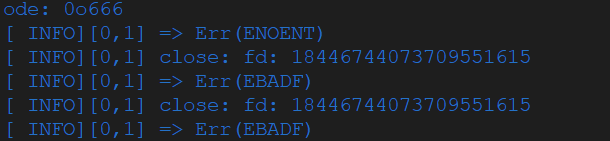
\includegraphics[width=\linewidth]{assets/syscall0.png}
        % \caption{}
        % \label{}
    \end{figure}
\end{frame}
    
\begin{frame}{小组分工}
    \begin{itemize}
        \item 罗崚骁
        \begin{itemize}
            \setlength{\itemsep}{8pt}
            \item 实现和完善系统调用
            \item 完成对 Git 支持
            \item 完成对 cargo 离线版的支持
            \item 测试 C++ 和 Rust 项目
        \end{itemize}
        \item 宋香君
        \begin{itemize}
            \setlength{\itemsep}{8pt}
            \item 实现和完善系统调用
            \item 完成对 make,CMake 的支持
            \item 测试 C 项目
        \end{itemize}
    \end{itemize}
\end{frame}

\begin{frame}{结束}
    谢谢观看
\end{frame}

\end{document}
